\section{Das Problem des Handlungsreisenden als Beispielanwendungsfall}\label{chap:TSP}

Dieser Algorithmus wird heute immer noch häufig für verschiedene Problemstellungen verwendet. Bekannte Anwendungsfälle sind \citep[S.9]{Blum2003}:
\begin{itemize}
  \item Busrouten, Müllabfuhr, Post- und Auslieferungsrouten
  \item Maschinenbelegungsproblem: Minimierung der Transportzeit bei räumlich weit auseinander liegenden Produktionsstätten
  \item Routenoptimierung zur Nachschubversorgung von Fertigungslinien mit minimalem Transportmitteleinsatz 
  \item 2D HP Proteinfaltung
  \item Beschickung von Lackieranlagen
  \item Fertigungssteuerung
  \item Telefonnetzwerk und Internet
  \item Personaleinsatzplanung
  \item Optimale Steuerung und Auslastung von Fahrzeugen und Fahrwegen
  
\end{itemize}
Ein sehr bekannter Anwendungsfall ist das Traveling Salesman Problem. Hierbei geht es um eine Optimierung in dem Bereich der Routenoptimierung. Ein Händler möchte mehrere Städte in so kurzer Zeit wie möglich besuchen und dann wieder zu seinem Ausgangspunkt zurückkehren \citep[S.37]{OKWU.2021}.
\newline
\newline
Dieses Problem wird auch in dem Shiny-Dashboard dargestellt und gezeigt, wie sich die Ergebnisse bei verschiedenen Einstellungen der Parameter ändert. Die Anzahl und die Orte der Städte bleiben dabei immer gleich, sodass man die Unterschiede durch die Parameter direkt sehen kann.
\newline
Auf dem Dashboard sieht man ein Koordinatensystem mit mehreren Slidern an der Seite und zwei ActionButtons. Die Funktionen für den Plot, die Slider und die Buttons werden in dem SKript mod-tsp-tab festgelegt. Auch die Server Funktionen sind in diesem Skript zu finden.
\begin{figure}[H]
 \centering
 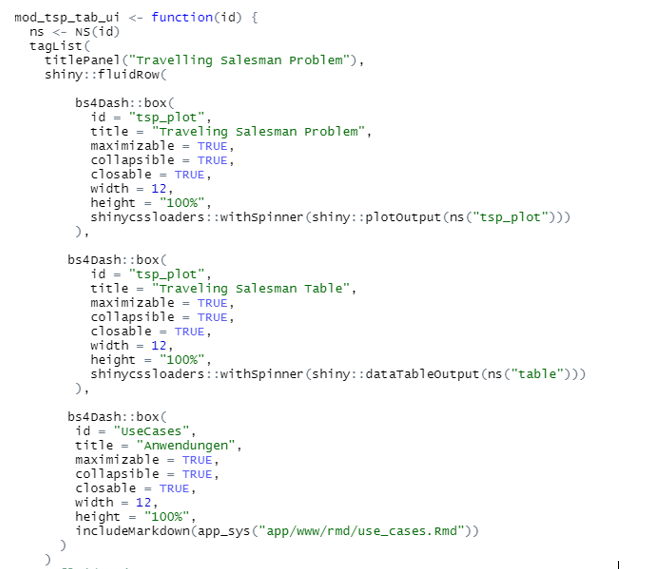
\includegraphics[scale=.7]{"images/05_Tsp/ui_mod_tsp_tab.png"}
 \caption{Quellcode für die UI Funktion des TSP Tabs}
 \label{fig:ui_mod_tsp_tab}
\end{figure}

\begin{figure}[H]
 \centering
 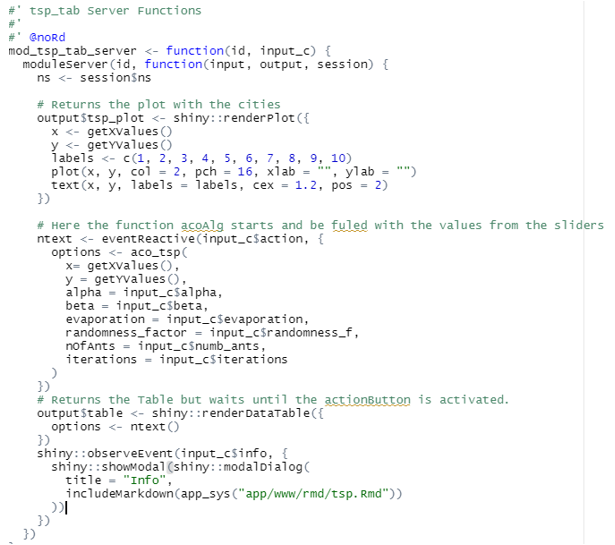
\includegraphics[scale=.7]{"images/05_Tsp/server_mod_tsp_tab.png"}
 \caption{Quellcode für die Server Funktion des TSP Tabs}
 \label{fig:server_mod_tsp_tab}
\end{figure}
Die erste Funktion im Server: output\$TSPlot ist zuständig für die Ausgabe des Plots.
\newline 
In unserem Beispiel wird mit 10 Städten gerechnet. Die X-, und Y-Werte werden über die Funktionen getXValues() und getYValues() gezogen. Diese Werte bleiben auch immer gleich. Mit der Abbildung kann man selbst immer die ausgegebenen Wege des ACO-Algorithmus nachgehen und entscheiden, ob die Lösung des Algorithmus eine Gute ist oder nicht.
\newline
In dem Shiny-Dashboard kann der Benutzer selbständig die Parameter über mehrere Slider an der Seite bestimmen und über einen Action-Button die Funktion des ACO mit den Slider-Parametern aufrufen. In der Funktion ntext <- eventReactive() wird der ACO mit den Werten der Slider befüllt und dann aufgerufen. Es werden wieder die X-, und Y-Werte mit den zwei Funktionen übergeben. Der Algorithmus wartet mit dem Aufruf der Funktion solange, bis der Benutzer auf den ActionButton klickt. 
\newline 
Im Folgenden wir dann das Ergebnis berechnet und über eine Tabelle ausgegeben, die immer alle minimalen Ruten enthält. Dabei kommt es häufig vor, dass der Algorithmus das minimale Ergebnis nicht nur einmal, sondern öfters findet und dann auch in der Tabelle ausgibt. Die Tabelle wird im Server in der Funktion output\$table <- renderDataTable() aufgerufen, sobald der ACO seine Berechnungen erledigt hat. Anhand der Distance in der Tabelle kann man sehen, ob der Algorithmus eine bessere oder schlechtere Route gefunden hat als davor.
\begin{figure}[H]
 \centering
 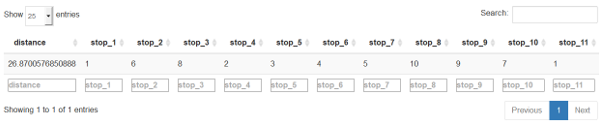
\includegraphics[scale=.7]{"images/05_Tsp/tsp_tabelle.png"}
 \caption{Tabelle mit den Ergebnissen des TSP}
 \label{fig:tsp_tabelle}
\end{figure}
Die Slider, der Plot und die Tabelle werden in der UI festgelegt und mit Min-, Max- und Anfangswerten versehen. Die Intervalle der Slider kann man dadurch schnell anpassen und auch größere Rechnungen durchführen, wenn man das möchte. Für die größeren Rechnungen muss man auch mehr Zeit einplanen. Hier ist der Action Button wichtig, der für die Ausführung des ACO -Algorithmus zuständig ist. Ohne ihn würde der Algorithmus bei jeder Änderung eines Slider und direkt beim Starten des Dashboards ausgeführt werden, das führt dann zu langen Wartezeiten und man kann nicht mehrere Parameter für seine Versuche mit dem Algorithmus verändern. 
\newline
\newline
Der Algorithmus, der das TSP durchführt ist von dem  \href {https://github.com/ciessielski/ACOTSP} {Git-Repository}. Dabei wurden kleine Änderungen gemacht, wie das Verändern der festen Parameter über die Slider. 
\newline
Der ACO Algorithmus wird über die Funktion aco-tsp ausgeführt.
\begin{figure}[h]
 \centering
 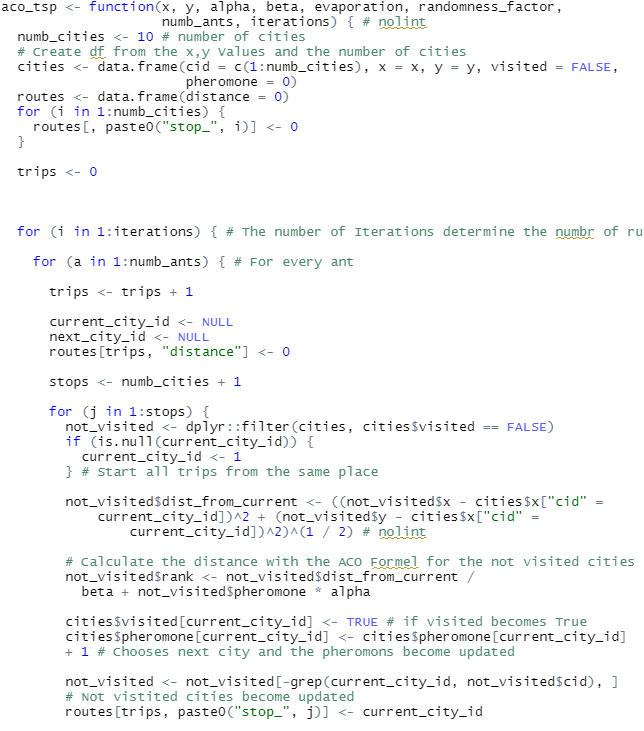
\includegraphics[scale=.6]{"images/05_Tsp/fct_aco_tsp1.png"}
 \caption{Quellcode zu TSP ACO Function}
 \label{actionButtonPhasen}
\end{figure}
\begin{figure}[h]
 \centering
 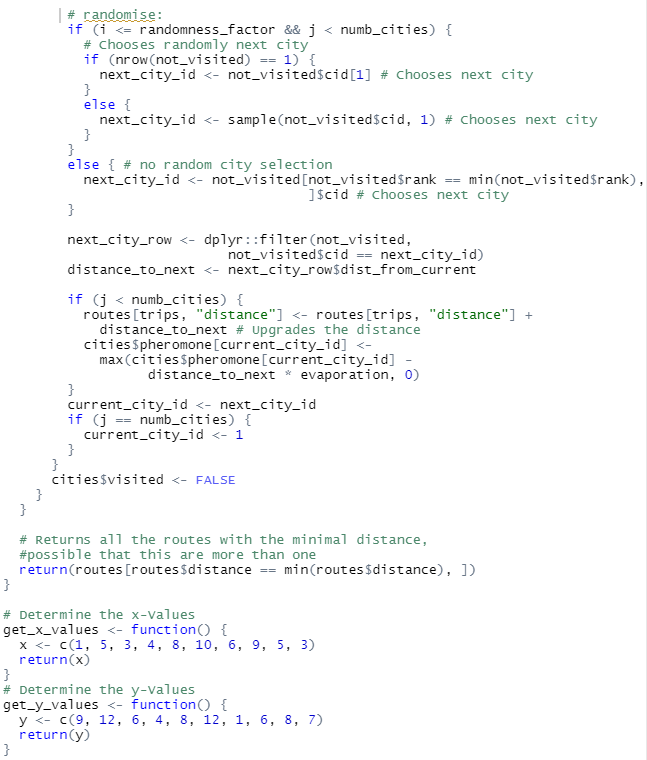
\includegraphics[scale=.6]{"images/05_Tsp/fct_aco_tsp2.png"}
 \caption{Quellcode zu TSP ACO Function}
 \label{actionButtonPhasen}
\end{figure}

Am Anfang des Codes werden die Parameter übergeben und ein Data Frame aus den X- und Y-Werten erstellt. Anhand der Anzahl der Städte wird die Anzahl an Stopps berechnet. Diese muss um eins höher sein als die Anzahl der Städte.
\newline
Für jede angegebene Iteration werden nun die einzelnen Schritte durchgeführt. Dabei durchläuft jede Ameise einen bestimmten Durchlauf. Bei jedem Durchlauf wird eine Route erstellt. Bei jeder Route ist das Ziel eine Distanz aufzunehmen und am Ende von allen Distanzen die Minimale mit ihren Stopps in der Reihenfolge auszugeben.
\newline
Jede Ameise beginnt bei der gleichen Stadt. Das wird direkt am Anfang der For-Schleife bei den Stopps festgelegt. Danach werden alle Distanzen zu den anderen Städten berechnet und den noch nicht besichtigten Städten einen Rang gegeben. Der Rang setzt sich aus der mathematischen Formel des ACO Algorithmus von Beta, Pheromonen und Alpha zusammen. Danach wird der Status der Stadt auf besichtigt gesetzt und die nächste Stadt in der Route ausgewählt. Die Auswahl der nächsten Route kann auch zufällig passieren, je nachdem wie hoch der Randomness-factor gesetzt wurde. Nach der Auswahl der nächsten Stadt, wird die Pheromonspur der Strecke von der aktuellen Stadt und der nächsten Stadt erhöht aber auch mit der Verdunstung verrechnet. Danach wird dasselbe mit der nächsten Stadt gemacht, nur dass es diesmal eine Möglichkeit weniger gibt, die die Ameisen wählen kann, da eine Stadt nur einmal besichtigt werden kann. 
\newline
Nachdem alle Städte abgelaufen wurden, wird die nächste Ameise ausgewählt. Sobald alle Ameisen ihre Routen gelaufen sind, wird alles nochmal ausgeführt, bis die Anzahl an Iterationen erreicht ist.
\newline
Jede Tour von jeder Ameise wird dabei in einer Tabelle mit der Distanz der Ameise gespeichert. Am Ende werden dann alle Routen mit der minimalen Distanz ausgegeben. 
\newline
\newline
Der Ameisenalgorithmus findet auch heute noch seine Anwendungen und ist sehr beliebt, wenn es um das schnelle Finden von einer guten Lösung geht. Es wird aber nicht immer die beste Lösung gefunden, außerdem ist es für den ACO beinahe unmöglich, eine noch bessere Route zu finden, wenn er schon eine sehr gute gefunden hat. Das schließt dann auch die Anwendung des ACO aus, wenn die Aufgabe besteht eine genaue und ideale Lösung zu finden \citep{LogistikInfonodate}.
\newline
\newline
Weitere Nachteile des Ameisenalgorithmus sind seine Komplexität und seine Ungenauigkeit. Den Ameisenalgorithmus manuell durchzuführen ist beinahe unmöglich und daher auch nur mit einem Computer machbar. Es ist außerdem wichtig für den ACO-Algorithmus, dass die Probleme als Graphen dargestellt werden müssen, damit Lösungen konstruierbar sind.
\newline
\newline
Trotz allem wird der Ameisenalgorithmus sehr gerne in der Logistik angewandt, da dort eine gute Lösung sehr häufig reicht, um sehr viel Geld oder Zeit zu sparen. Es ist daher in der Logistik nicht notwendig, immer die beste Lösung zu finden \citep{LogistikInfonodate}.
